%==============================================================
%  EE201 -- Circuit Theory I
%  Lecture 14 : Two-Port Circuits
%  M. Mert Ankaralı, METU EEE
%
%  Compile:  ./build.sh      (or: pdflatex EE201_Lecture_14.tex, twice)
%==============================================================
\documentclass[11pt,a4paper]{article}

%-------------------- packages --------------------------------
\usepackage[T1]{fontenc}
\usepackage[utf8]{inputenc}
\usepackage[english]{babel}
\usepackage{lmodern}
\usepackage[left=2.2cm,right=4.4cm,top=2.2cm,bottom=2.2cm,headheight=14pt,headsep=9pt,marginparwidth=3.4cm,marginparsep=0.5cm]{geometry}
\usepackage{amsmath,amssymb}
\usepackage{array,booktabs,tabularx}
\usepackage{enumitem}
\usepackage{needspace}
\usepackage[table]{xcolor}
\usepackage{fancyhdr}
\usepackage{titlesec}
\usepackage{graphicx}
\usepackage[most]{tcolorbox}
\usepackage{tikz}
\usepackage[american,siunitx]{circuitikz}
\usetikzlibrary{matrix,arrows.meta,positioning,calc,decorations.pathmorphing,decorations.pathreplacing,decorations.markings,patterns,shapes.geometric}
\usepackage[colorlinks=true,allcolors=metured,breaklinks=true]{hyperref}

%-------------------- colour system ---------------------------
% One colour per physical quantity, used identically in the slides.
\definecolor{metured}{RGB}{155,27,48}    % headings, structure
\definecolor{metugray}{RGB}{88,89,91}
\definecolor{ccur}{RGB}{0,102,170}       % CURRENT  -- blue
\definecolor{cvolt}{RGB}{214,120,0}      % VOLTAGE  -- orange
\definecolor{cpow}{RGB}{23,128,74}       % POWER / ENERGY -- green
\definecolor{ccharge}{RGB}{124,60,160}   % CHARGE   -- purple
\definecolor{cflux}{RGB}{0,138,138}      % FLUX -- teal
\definecolor{boxgray}{RGB}{245,245,245}
\definecolor{copper}{RGB}{184,98,30}

\newcommand{\Icol}[1]{\textcolor{ccur}{#1}}
\newcommand{\Vcol}[1]{\textcolor{cvolt}{#1}}
\newcommand{\Pcol}[1]{\textcolor{cpow}{#1}}
\newcommand{\Qcol}[1]{\textcolor{ccharge}{#1}}
\newcommand{\Fcol}[1]{\textcolor{cflux}{#1}}

%-------------------- units (no siunitx dependency) -----------
\newcommand{\uni}[1]{\,\mathrm{#1}}
\newcommand{\A}{\uni{A}}   \newcommand{\V}{\uni{V}}
\newcommand{\W}{\uni{W}}   \newcommand{\J}{\uni{J}}
\newcommand{\Cb}{\uni{C}}  \newcommand{\s}{\uni{s}}
\newcommand{\Sie}{\uni{S}} \newcommand{\Wb}{\uni{Wb}}

%-------------------- layout ----------------------------------
\pagestyle{fancy}
\fancyhf{}
\lhead{\small\textcolor{metugray}{EE201 -- Circuit Theory I}}
\rhead{\small\textcolor{metugray}{Lecture 14: Two-Port Circuits}}
\cfoot{\small\thepage}
\renewcommand{\headrulewidth}{0.4pt}

\titleformat{\section}{\large\bfseries\color{metured}}{\thesection.}{0.6em}{}
\titleformat{\subsection}{\normalsize\bfseries\color{metugray}}{\thesubsection.}{0.6em}{}
\titlespacing*{\section}{0pt}{1.4ex plus .3ex}{0.7ex}
\titlespacing*{\subsection}{0pt}{1.1ex plus .2ex}{0.5ex}

\setlist[itemize]{itemsep=2pt,topsep=3pt,parsep=0pt,leftmargin=1.5em}
\setlist[enumerate]{itemsep=2pt,topsep=3pt,parsep=0pt,leftmargin=1.7em}
\setlength{\parindent}{0pt}
\setlength{\parskip}{1.2ex plus .2ex}
\linespread{1.25}
\AtBeginDocument{\setlength{\abovedisplayskip}{12pt plus 3pt}\setlength{\belowdisplayskip}{12pt plus 3pt}}
\raggedbottom
\widowpenalty=10000
\clubpenalty=10000
\brokenpenalty=10000

%-------------------- boxes -----------------------------------
\newtcolorbox{definitionbox}[1]{enhanced,
  colback=metured!4, colframe=metured, boxrule=0.9pt,
  fonttitle=\bfseries, title={#1}, arc=2pt,
  left=7pt,right=7pt,top=5pt,bottom=5pt, before skip=7pt, after skip=7pt,
  before upper={\setlength{\parskip}{0.6ex plus .1ex}}}

\newtcolorbox{ideabox}[1][Key idea]{enhanced,
  colback=ccur!5, colframe=ccur, boxrule=0.9pt,
  fonttitle=\bfseries, title={#1}, arc=2pt,
  left=7pt,right=7pt,top=5pt,bottom=5pt, before skip=7pt, after skip=7pt,
  before upper={\setlength{\parskip}{0.6ex plus .1ex}}}

\newtcolorbox{examplebox}[1][Example]{enhanced,
  colback=cpow!4, colframe=cpow, boxrule=0.9pt,
  fonttitle=\bfseries, title={#1}, arc=2pt,
  left=7pt,right=7pt,top=5pt,bottom=5pt, before skip=7pt, after skip=7pt,
  before upper={\setlength{\parskip}{0.6ex plus .1ex}}}

%  Example solutions: a heading and numbered steps outside the example box
\newif\ifsolfirst
\newcommand{\solution}{\par\smallskip\noindent{\color{cpow}\bfseries Solution}\par\nobreak\smallskip\global\solfirsttrue}
\newcommand{\solstep}[2]{\par\ifsolfirst\global\solfirstfalse\else\bigskip\needspace{5\baselineskip}\fi
  \noindent{\color{cpow}\bfseries Step #1.}\ {\bfseries #2}\par\nobreak\smallskip}

\newtcolorbox{cautionbox}[1][Careful]{enhanced,
  colback=cvolt!6, colframe=cvolt, boxrule=0.9pt,
  fonttitle=\bfseries, title={#1}, arc=2pt,
  left=7pt,right=7pt,top=5pt,bottom=5pt, before skip=7pt, after skip=7pt,
  before upper={\setlength{\parskip}{0.6ex plus .1ex}}}

%-------------------- circuitikz defaults ---------------------
%  voltage sources: smaller + and - inside the circle, further apart
\ctikzset{bipoles/vsourceam/inner plus={\tiny$+$},
          bipoles/vsourceam/inner minus={\tiny$\vphantom{+}-$},
          bipoles/vsourceam/margin=0.85,
          bipoles/cvsourceam/inner plus={\tiny$+$},
          bipoles/cvsourceam/inner minus={\tiny$\vphantom{+}-$},
          bipoles/cvsourceam/margin=0.85}
\ctikzset{bipoles/length=0.9cm, color=black,
          label/align=straight,
          bipoles/generic/height=0.28, bipoles/generic/width=0.62}
\tikzset{
  iar/.style={-{Stealth[length=2.2mm]}, ccur, thick},
  pol/.style={font=\small, text=cvolt},
  glab/.style={font=\footnotesize, text=metured},
  ttl/.style={font=\scriptsize\bfseries, text=metugray},
  capn/.style={font=\scriptsize, text=metugray, align=center},
  bigarr/.style={-{Stealth[length=3mm]}, very thick, metugray},
  gnode/.style={circle, fill=metured, inner sep=0pt, minimum size=4.4pt},
  nlab/.style={circle, draw=metured, text=metured, font=\scriptsize, inner sep=0.7pt},
  blab/.style={font=\footnotesize, text=black!80},
  gbr/.style={black!75, thick, postaction={decorate, decoration={markings,
      mark=at position 0.56 with {\arrow{Stealth[length=2.5mm]}}}}},
  apbr/.style={ccur, line width=1.7pt, postaction={decorate, decoration={markings,
      mark=at position 0.56 with {\arrow{Stealth[length=2.8mm]}}}}},
  hal/.style={draw=cpow!60, line width=6pt, opacity=0.35, line cap=round, line join=round},
  elem/.style={draw=metugray, thick, fill=metulight},
}
\definecolor{metulight}{RGB}{243,240,241}

%-------------------- Lecture 14 circuit macros ---------------
\newcommand{\ohm}{\,\Omega}
\newcommand{\yes}{\textcolor{cpow}{\checkmark}}
\newcommand{\e}[1]{\textcolor{cvolt}{e_{#1}}}
\newcommand{\nd}[1]{\tikz[baseline=(c.base)]\node[nlab](c){#1};}
\newcommand{\gnd}[2]{\draw (#1,#2) -- ++(0,-0.2) node[ground] {};}
\newcommand{\Rin}{R_{\mathrm{in}}}
%  Port variables in colour
\newcommand{\vone}{\Vcol{v_1}}  \newcommand{\vtwo}{\Vcol{v_2}}
\newcommand{\ione}{\Icol{i_1}}  \newcommand{\itwo}{\Icol{i_2}}
\newcommand{\Rm}{\mathbf{R}}  \newcommand{\Gm}{\mathbf{G}}
\newcommand{\Hm}{\mathbf{H}}  \newcommand{\Tm}{\mathbf{T}}
%  Labels beside a vertical element at (#1,#2), a fixed distance to the right (\lR) or left (\lL)
\newcommand{\lR}[3]{\node[anchor=west, xshift=7pt, font=\small] at (#1,#2) {#3};}
\newcommand{\lL}[3]{\node[anchor=east, xshift=-7pt, font=\small] at (#1,#2) {#3};}
\tikzset{tlab/.style={font=\small\bfseries, text=black!80},
         dotm/.style={circle, fill=black, inner sep=0pt, minimum size=4.2pt},
         core/.style={line width=1.1pt, metugray}}

%  Port 1 at terminals x = #1 (top y = #2, bottom y = 0): i_1 into the top terminal, + v_1 -
\newcommand{\pone}[2]{%
  \draw (#1,#2) node[ocirc] {}; \draw (#1,0) node[ocirc] {};
  \draw[iar] (#1+0.2,#2+0.28) -- (#1+0.75,#2+0.28); \node[font=\small, text=ccur] at (#1+0.48,#2+0.58) {$i_1$};
  \node[pol] at (#1+0.3,0.72*#2) {$+$}; \node[pol] at (#1+0.3,0.22*#2) {$-$};
  \node[font=\small, text=cvolt] at (#1+0.32,0.47*#2) {$v_1$};}
%  Port 2 at terminals x = #1: i_2 into the top terminal (pointing left), + v_2 -
\newcommand{\ptwo}[2]{%
  \draw (#1,#2) node[ocirc] {}; \draw (#1,0) node[ocirc] {};
  \draw[iar] (#1-0.2,#2+0.28) -- (#1-0.75,#2+0.28); \node[font=\small, text=ccur] at (#1-0.48,#2+0.58) {$i_2$};
  \node[pol] at (#1-0.3,0.72*#2) {$+$}; \node[pol] at (#1-0.3,0.22*#2) {$-$};
  \node[font=\small, text=cvolt] at (#1-0.32,0.47*#2) {$v_2$};}
%  A two-port box (text #1) with both ports
\newcommand{\tpbox}[1]{%
  \draw[elem] (1.0,-0.2) rectangle (3.4,2.2);
  \node[align=center, font=\small] at (2.2,1.0) {#1};
  \draw (0,1.8) -- (1.0,1.8); \draw (0,0) -- (1.0,0);
  \draw (3.4,1.8) -- (4.4,1.8); \draw (3.4,0) -- (4.4,0);
  \pone{0}{1.8} \ptwo{4.4}{1.8}}
%  A one-port box with a resistor-like port (for the review)
\newcommand{\opbox}[1]{%
  \draw[elem] (0,0) rectangle (1.9,2);
  \node[align=center, font=\small] at (0.95,1) {#1};
  \draw (1.9,1.7) -- (3.0,1.7) node[ocirc] {}; \draw (1.9,0.3) -- (3.0,0.3) node[ocirc] {};
  \draw[iar] (2.75,1.95) -- (2.2,1.95); \node[font=\small, text=ccur] at (2.48,2.25) {$i$};
  \node[pol] at (2.6,1.4) {$+$}; \node[pol] at (2.6,0.6) {$-$};
  \node[font=\small, text=cvolt] at (2.6,1.0) {$v$};}

%  Example 14.1: R_1 across port 1, R_2 across port 2 (no coupling)
\newcommand{\exTriv}{%
  \draw (0,1.8) -- (1.5,1.8); \draw (0,0) -- (1.5,0);
  \draw (1.5,1.8) to[R] (1.5,0); \lR{1.5}{0.9}{$2\ohm$}
  \draw (4.1,1.8) to[R] (4.1,0); \lL{4.1}{0.9}{$4\ohm$}
  \draw (4.1,1.8) -- (5.6,1.8); \draw (4.1,0) -- (5.6,0);
  \draw[dashed, metugray] (1.0,-0.45) rectangle (4.6,2.45);
  \pone{0}{1.8} \ptwo{5.6}{1.8}}

%  Example 14.2: R_1 (series), R_2 (shunt), CCVS 2 i_1 (+ on the left).
%  #1 = 0: both ports;  1: i_2 = 0 (port 2 open);  2: i_1 = 0 (port 1 open);  3: v_2 = 0 (port 2 shorted)
%  #2, #3: labels of R_1, R_2
\newcommand{\exTee}[4][2]{%
  \draw (0,2.2) -- (0.9,2.2) to[R, l=#3] (2.6,2.2) -- (4.3,2.2);
  \draw (4.3,2.2) to[american controlled voltage source, l=$\Vcol{#1\,i_1}$] (5.9,2.2) -- (6.9,2.2);
  \draw (2.6,2.2) to[R] (2.6,0); \lR{2.6}{1.1}{#4}
  \draw (0,0) -- (6.9,0);
  \fill (2.6,2.2) circle (1.7pt); \fill (2.6,0) circle (1.7pt);
  \ifcase#2
    \pone{0}{2.2} \ptwo{6.9}{2.2}
  \or
    \pone{0}{2.2}
    \draw (6.9,2.2) node[ocirc] {}; \draw (6.9,0) node[ocirc] {};
    \node[pol] at (6.6,1.6) {$+$}; \node[pol] at (6.6,0.5) {$-$};
    \node[font=\small, text=cvolt] at (6.58,1.05) {$v_2$};
    \node[font=\small, text=ccur, anchor=west] at (7.05,2.2) {$i_2 = 0$};
  \or
    \draw (0,2.2) node[ocirc] {}; \draw (0,0) node[ocirc] {};
    \node[pol] at (0.3,1.6) {$+$}; \node[pol] at (0.3,0.5) {$-$};
    \node[font=\small, text=cvolt] at (0.32,1.05) {$v_1$};
    \node[font=\small, text=ccur, anchor=east] at (-0.15,2.2) {$i_1 = 0$};
    \ptwo{6.9}{2.2}
  \or
    \pone{0}{2.2}
    \draw (6.9,2.2) -- (6.9,0);
    \draw[iar] (6.65,2.5) -- (6.1,2.5); \node[font=\small, text=ccur] at (6.38,2.8) {$i_2$};
    \node[font=\small, text=cvolt, anchor=west] at (7.05,1.1) {$v_2 = 0$};
  \fi}

%  Ideal transformer N_1 : N_2 as a two-port (coils at x = 1.4 and 3.0, height 1.8)
\newcommand{\xfmr}[2]{%
  \begin{scope}[xshift=#1 cm]
    \ctikzset{bipoles/length=1.2cm}
    \draw (0,0) to[L] (0,#2);
    \draw (1.6,#2) to[L] (1.6,0);
    \draw[core] (0.72,-0.05) -- (0.72,#2+0.05);
    \draw[core] (0.88,-0.05) -- (0.88,#2+0.05);
    \node[dotm] at (0.36,#2-0.2) {};
    \node[dotm] at (1.24,#2-0.2) {};
  \end{scope}}
\newcommand{\exXf}{%
  \draw (0,1.8) -- (1.4,1.8); \draw (0,0) -- (1.4,0);
  \xfmr{1.4}{1.8}
  \draw (3.0,1.8) -- (4.4,1.8); \draw (3.0,0) -- (4.4,0);
  \node[font=\small] at (2.2,2.2) {$N_1 : N_2$};
  \pone{0}{1.8} \ptwo{4.4}{1.8}}
\newcommand{\Rth}{R_{\mathrm{th}}}

%  Meters drawn upright: vertical (x, ytop, ybot, letter, label right) and horizontal (xl, xr, y, letter, label above)
\newcommand{\vmeter}[5]{%
  \draw (#1,#2) -- (#1,{(#2+#3)/2+0.32}); \draw (#1,{(#2+#3)/2-0.32}) -- (#1,#3);
  \node[circle, draw, thick, minimum size=0.64cm, inner sep=0pt, font=\small\bfseries] at (#1,{(#2+#3)/2}) {#4};
  \node[anchor=west, font=\small] at ({#1+0.38},{(#2+#3)/2}) {#5};}
\newcommand{\hmeter}[5]{%
  \draw (#1,#3) -- ({(#1+#2)/2-0.32},#3); \draw ({(#1+#2)/2+0.32},#3) -- (#2,#3);
  \node[circle, draw, thick, minimum size=0.64cm, inner sep=0pt, font=\small\bfseries] at ({(#1+#2)/2},#3) {#4};
  \node[anchor=south, font=\small] at ({(#1+#2)/2},{#3+0.36}) {#5};}
%  Test bench for a two-port in a box. #1 = 0: open-circuit test (current source at port 1,
%  voltmeters at both ports); 1: short-circuit test (voltage source at port 1, ammeters)
\newcommand{\bench}[1]{%
  \draw[thick, fill=gray!8] (3.0,-0.2) rectangle (5.0,2.4);
  \node[font=\large] at (4.0,1.1) {$N$};
  \draw (3.0,2.0) -- (2.6,2.0); \draw (3.0,0.2) -- (2.6,0.2);
  \draw (5.0,2.0) -- (5.4,2.0); \draw (5.0,0.2) -- (5.4,0.2);
  \foreach \p in {(2.6,2.0),(2.6,0.2),(5.4,2.0),(5.4,0.2)} \draw \p node[ocirc] {};
  \ifcase#1
    \draw (0,0.2) to[american current source, l=$\Icol{i_1}$] (0,2.0) -- (2.6,2.0);
    \draw (0,0.2) -- (2.6,0.2);
    \vmeter{1.5}{2.0}{0.2}{V}{$\Vcol{v_1}$}
    \fill (1.5,2.0) circle (1.6pt); \fill (1.5,0.2) circle (1.6pt);
    \draw (5.4,2.0) -- (6.6,2.0); \draw (5.4,0.2) -- (6.6,0.2);
    \vmeter{6.6}{2.0}{0.2}{V}{$\Vcol{v_2}$}
    \node[font=\small, text=ccur, anchor=south] at (6.0,2.05) {$i_2 = 0$};
  \or
    \draw (0,2.0) to[american voltage source, l_=$\Vcol{v_1}$] (0,0.2);
    \hmeter{0}{2.6}{2.0}{A}{$\Icol{i_1}$}
    \draw (0,0.2) -- (2.6,0.2);
    \draw (5.4,2.0) -- (6.6,2.0); \draw (5.4,0.2) -- (6.6,0.2);
    \vmeter{6.6}{2.0}{0.2}{A}{$\Icol{i_2}$}
    \node[font=\small, text=cvolt, anchor=south] at (6.0,2.05) {$v_2 = 0$};
  \fi}
\begin{document}

%-------------------- title block -----------------------------
\begin{center}
\begin{tcolorbox}[enhanced, colback=metured!5, colframe=metured, boxrule=1pt,
                  arc=3pt, left=10pt,right=10pt,top=7pt,bottom=7pt, width=\textwidth]
\begin{center}
  {\small\scshape Middle East Technical University}\\[2pt]
  {\small\scshape Department of Electrical and Electronics Engineering}\\[7pt]
  {\Large\bfseries\color{metured} EE201 -- Circuit Theory I}\\[4pt]
  {\large\bfseries Lecture 14: Two-Port Circuits}\\[6pt]
  {\small M. Mert Ankaral{\i}}
\end{center}
\end{tcolorbox}
\end{center}
\vspace{-0.5em}

\begin{center}
\small
\begin{tabular}{@{}l@{}}
\toprule
\textbf{Colour code used in these notes and in the slides}\\
\midrule
\Icol{$\blacksquare$}~current $i$ \quad
\Vcol{$\blacksquare$}~voltage $v$, node voltage $e$\\
\bottomrule
\end{tabular}
\end{center}

\textbf{Motivation.} Previously, a one-port without independent sources was described by one
number, its input resistance: $\Vcol{v} = \Rin\,\Icol{i}$. Many circuits have an input and an
output: an amplifier, a transformer, a filter. Such a circuit has two ports, and its
description is the natural generalization of $\Vcol{v} = R\,\Icol{i}$: two port voltages, two
port currents and a $2 \times 2$ matrix. This lecture introduces four such matrices
(\textbf{resistance}, \textbf{conductance}, \textbf{hybrid} and \textbf{transmission}) and the
\textbf{power} of a two-port.

%==============================================================
\section{Two-port circuits}

\begin{minipage}[c]{0.46\linewidth}
\centering
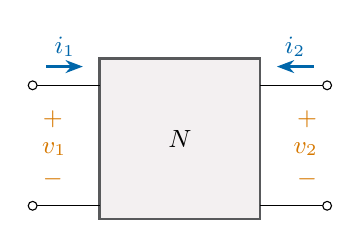
\begin{tikzpicture}[scale=0.85]
  \tpbox{$N$}
\end{tikzpicture}
\end{minipage}\hfill
\begin{minipage}[c]{0.5\linewidth}
$N$ is an LTI resistive circuit with no independent sources. At each port the current enters
at the $+$ terminal and leaves at the $-$ terminal. There are four port variables
$\vone$, $\ione$, $\vtwo$, $\itwo$ and two equations between them: two of the variables can
be written in terms of the other two.
\end{minipage}

\begin{center}
\small
\renewcommand{\arraystretch}{1.25}
\begin{tabular}{@{}llll@{}}
\toprule
\textbf{given} & \textbf{find} & \textbf{matrix} & \textbf{equation}\\
\midrule
$\ione$, $\itwo$ & $\vone$, $\vtwo$ & resistance $\Rm$ & $[\,\vone \ \vtwo\,]^T = \Rm\,[\,\ione \ \itwo\,]^T$\\
$\vone$, $\vtwo$ & $\ione$, $\itwo$ & conductance $\Gm$ & $[\,\ione \ \itwo\,]^T = \Gm\,[\,\vone \ \vtwo\,]^T$\\
$\ione$, $\vtwo$ & $\vone$, $\itwo$ & hybrid $\Hm$ & $[\,\vone \ \itwo\,]^T = \Hm\,[\,\ione \ \vtwo\,]^T$\\
$\vone$, $\itwo$ & $\ione$, $\vtwo$ & hybrid $\Hm'$ & $[\,\ione \ \vtwo\,]^T = \Hm'\,[\,\vone \ \itwo\,]^T$\\
$\vtwo$, $-\itwo$ & $\vone$, $\ione$ & transmission $\Tm$ & $[\,\vone \ \ione\,]^T = \Tm\,[\,\vtwo \ {-\itwo}\,]^T$\\
\bottomrule
\end{tabular}
\end{center}

%==============================================================
\section{The resistance matrix}

\begin{definitionbox}{Resistance matrix}
\begin{minipage}[c]{0.5\linewidth}
The port voltages in terms of the port currents:
\[
  \begin{aligned}
    \vone &= r_{11}\,\ione + r_{12}\,\itwo\\
    \vtwo &= r_{21}\,\ione + r_{22}\,\itwo
  \end{aligned}
\]
\end{minipage}\hfill
\begin{minipage}[c]{0.46\linewidth}
\[
  \begin{bmatrix} \vone\\ \vtwo \end{bmatrix}
  = \underbrace{\begin{bmatrix} r_{11} & r_{12}\\ r_{21} & r_{22} \end{bmatrix}}_{\Rm}
    \begin{bmatrix} \ione\\ \itwo \end{bmatrix}
\]
\end{minipage}
\end{definitionbox}

\medskip
\begin{examplebox}[Example 14.1 --- two separate resistors]
\begin{minipage}[c]{0.5\linewidth}
\centering
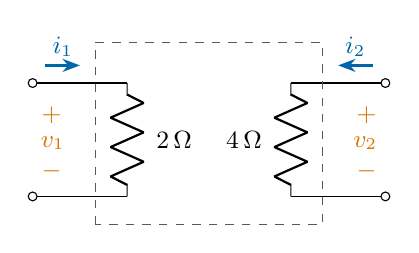
\begin{tikzpicture}[scale=0.8]
  \exTriv
\end{tikzpicture}
\end{minipage}\hfill
\begin{minipage}[c]{0.46\linewidth}
The two-port is a $2\ohm$ resistor across port 1 and a $4\ohm$ resistor across port 2. Find
$\Rm$.
\end{minipage}
\end{examplebox}

\solution

\solstep{1}{Each port alone}
Each resistor carries only its own port current:
\[
  \vone = 2\,\ione + 0 \cdot \itwo, \qquad \vtwo = 0 \cdot \ione + 4\,\itwo .
\]

\solstep{2}{The matrix}
\[
  \Rm = \begin{bmatrix} 2 & 0\\ 0 & 4 \end{bmatrix}\,\Omega .
\]
The off-diagonal entries are zero: the two ports are not coupled.

\bigskip
\begin{examplebox}[Example 14.2 --- a dependent source inside]
\begin{center}
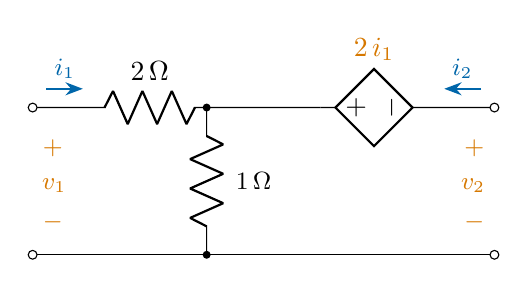
\begin{tikzpicture}[scale=0.85]
  \exTee{0}{$2\ohm$}{$1\ohm$}
\end{tikzpicture}
\end{center}
The two-port contains a $2\ohm$ and a $1\ohm$ resistor and a current-controlled voltage source $2\,\ione$.
Find $\Rm$.
\end{examplebox}

\solution

\solstep{1}{The current of $1\ohm$}
By KCL at the middle node, the $1\ohm$ resistor carries $\ione + \itwo$ downwards.

\solstep{2}{KVL from each port}
From port 1 through $2\ohm$ and $1\ohm$:
\[
  \vone = 2\,\ione + (\ione + \itwo) = 3\,\ione + \itwo .
\]
From port 2 through the dependent source and $1\ohm$:
\[
  \vtwo = -2\,\ione + (\ione + \itwo) = -\ione + \itwo .
\]

\solstep{3}{The matrix}
Collect the terms in $\ione$ and $\itwo$:
\[
  \Rm = \begin{bmatrix} 3 & 1\\ -1 & 1 \end{bmatrix}\Omega .
\]
Without the dependent source $\Rm$ would be symmetric; here $r_{12} \neq r_{21}$.

\subsection{The entries from open-circuit tests}

The matrix equation in the box above also tells how to find $\Rm$ one column
at a time: make one port current zero, that is, leave that port \textbf{open}.

\textbf{Port 2 open} ($\itwo = 0$). Drive port 1 with a current $\ione$, for example with a
current source. The second column of $\Rm$ is multiplied by zero and drops out:
\[
  \begin{bmatrix} \vone\\ \vtwo \end{bmatrix}
  = \begin{bmatrix} r_{11} & r_{12}\\ r_{21} & r_{22} \end{bmatrix}
    \begin{bmatrix} \ione\\ 0 \end{bmatrix}
  = \begin{bmatrix} r_{11}\,\ione\\ r_{21}\,\ione \end{bmatrix} .
\]
Both port voltages are proportional to $\ione$. Dividing by $\ione$ gives the
\textbf{first column}:
\[
  r_{11} = \frac{\vone}{\ione}\bigg|_{\itwo = 0}, \qquad
  r_{21} = \frac{\vtwo}{\ione}\bigg|_{\itwo = 0} .
\]

\textbf{Port 1 open} ($\ione = 0$). Drive port 2 with a current $\itwo$. Now the first column
drops out:
\[
  \begin{bmatrix} \vone\\ \vtwo \end{bmatrix}
  = \begin{bmatrix} r_{11} & r_{12}\\ r_{21} & r_{22} \end{bmatrix}
    \begin{bmatrix} 0\\ \itwo \end{bmatrix}
  = \begin{bmatrix} r_{12}\,\itwo\\ r_{22}\,\itwo \end{bmatrix} ,
\]
and dividing by $\itwo$ gives the \textbf{second column}:
\[
  r_{12} = \frac{\vone}{\itwo}\bigg|_{\ione = 0}, \qquad
  r_{22} = \frac{\vtwo}{\itwo}\bigg|_{\ione = 0} .
\]

\textbf{What the entries mean.} The diagonal entries are input resistances: $r_{11}$ is the
resistance seen at port 1 when port 2 is open, and $r_{22}$ is the resistance seen at port 2
when port 1 is open. The off-diagonal entries are transfer resistances: $r_{21}$ is the voltage
that appears at the open port 2 per ampere into port 1, and $r_{12}$ the other way round. Since
both tests leave a port open, $\Rm$ is also called the \textbf{open-circuit resistance matrix}.
Each test is an ordinary one-source linear circuit.

\medskip
\begin{examplebox}[Example 14.2 revisited --- open-circuit tests]
Find $\Rm$ of Example 14.2 again, this time from the two open-circuit tests.
\end{examplebox}

\solution

\solstep{1}{Port 2 open: $\itwo = 0$}
\begin{minipage}[c]{0.56\linewidth}
\centering
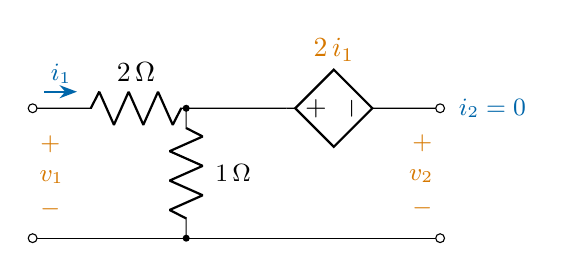
\begin{tikzpicture}[scale=0.75]
  \exTee{1}{$2\ohm$}{$1\ohm$}
\end{tikzpicture}
\end{minipage}\hfill
\begin{minipage}[c]{0.4\linewidth}
No current flows through the dependent source, so $\vtwo$ is the voltage of $1\ohm$ minus the dependent source:
\begin{align*}
  \vone &= (2 + 1)\,\ione = 3\,\ione\\
  \vtwo &= \ione - 2\,\ione = -\ione
\end{align*}
\end{minipage}

\smallskip
So $r_{11} = 3\ohm$ and $r_{21} = -1\ohm$.

\solstep{2}{Port 1 open: $\ione = 0$}
\begin{minipage}[c]{0.56\linewidth}
\centering
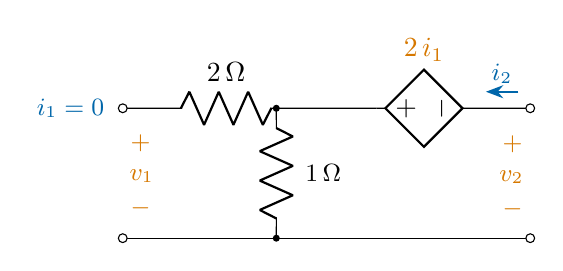
\begin{tikzpicture}[scale=0.75]
  \exTee{2}{$2\ohm$}{$1\ohm$}
\end{tikzpicture}
\end{minipage}\hfill
\begin{minipage}[c]{0.4\linewidth}
No current flows in $2\ohm$, and the dependent source is $2\,\ione = 0$:
\begin{align*}
  \vone &= \itwo\\
  \vtwo &= \itwo
\end{align*}
\end{minipage}

\smallskip
So $r_{12} = 1\ohm$ and $r_{22} = 1\ohm$: the same $\Rm$ as before. \ \yes

%==============================================================
\section{The conductance matrix}

\begin{definitionbox}{Conductance matrix}
\begin{minipage}[c]{0.46\linewidth}
The port currents in terms of the port voltages:
\[
  \begin{bmatrix} \ione\\ \itwo \end{bmatrix}
  = \underbrace{\begin{bmatrix} g_{11} & g_{12}\\ g_{21} & g_{22} \end{bmatrix}}_{\Gm}
    \begin{bmatrix} \vone\\ \vtwo \end{bmatrix} .
\]
\end{minipage}\hfill
\begin{minipage}[c]{0.5\linewidth}
The entries follow from \textbf{short-circuit tests}:
\[
  g_{11} = \frac{\ione}{\vone}\bigg|_{\vtwo = 0}, \quad
  g_{21} = \frac{\itwo}{\vone}\bigg|_{\vtwo = 0},
\]
\[
  g_{12} = \frac{\ione}{\vtwo}\bigg|_{\vone = 0}, \quad
  g_{22} = \frac{\itwo}{\vtwo}\bigg|_{\vone = 0} .
\]
\end{minipage}
\end{definitionbox}

\textbf{The entries, column by column.} Now make one port \emph{voltage} zero, that is,
\textbf{short} that port, and drive the other port with a voltage.

\smallskip
\noindent
\begin{minipage}[t]{0.49\linewidth}
\centering
\textbf{Port 2 shorted} ($\vtwo = 0$):
\[
  \begin{bmatrix} \ione\\ \itwo \end{bmatrix}
  = \begin{bmatrix} g_{11} & g_{12}\\ g_{21} & g_{22} \end{bmatrix}
    \begin{bmatrix} \vone\\ 0 \end{bmatrix}
  = \begin{bmatrix} g_{11}\,\vone\\ g_{21}\,\vone \end{bmatrix}
\]
the \textbf{first column}.
\end{minipage}\hfill
\begin{minipage}[t]{0.49\linewidth}
\centering
\textbf{Port 1 shorted} ($\vone = 0$):
\[
  \begin{bmatrix} \ione\\ \itwo \end{bmatrix}
  = \begin{bmatrix} g_{11} & g_{12}\\ g_{21} & g_{22} \end{bmatrix}
    \begin{bmatrix} 0\\ \vtwo \end{bmatrix}
  = \begin{bmatrix} g_{12}\,\vtwo\\ g_{22}\,\vtwo \end{bmatrix}
\]
the \textbf{second column}.
\end{minipage}

\medskip
\textbf{What the entries mean.} The diagonal entries are input conductances: $g_{11}$ is the
conductance seen at port 1 when port 2 is shorted, and $g_{22}$ the conductance seen at port 2
when port 1 is shorted. The off-diagonal entries are transfer conductances: $g_{21}$ is the
current that flows in the shorted port 2 per volt at port 1, and $g_{12}$ the other way round.
Since both tests short a port, $\Gm$ is also called the \textbf{short-circuit conductance
matrix}.

If $\Rm$ is invertible, $\mathbf{v} = \Rm\,\mathbf{i}$ gives $\mathbf{i} = \Rm^{-1}\mathbf{v}$, so
$\Gm = \Rm^{-1}$ (and $\Rm = \Gm^{-1}$). Note that $g_{11} \neq 1/r_{11}$ in general: the two
are measured with the other port shorted and open, respectively.

\bigskip
\begin{examplebox}[Example 14.3 --- the conductance matrix of Example 14.2]
Find the first column of $\Gm$ for the two-port of Example 14.2 by a short-circuit test. Then
find all of $\Gm$.
\end{examplebox}

\solution

\solstep{1}{Port 2 shorted: $\vtwo = 0$}
\begin{minipage}[c]{0.56\linewidth}
\centering
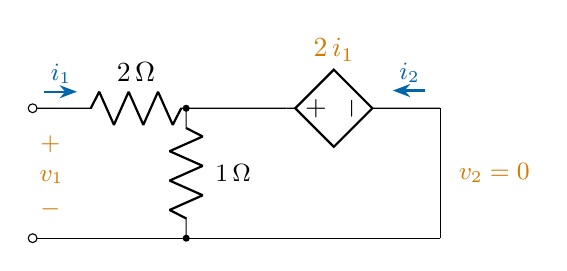
\begin{tikzpicture}[scale=0.75]
  \exTee{3}{$2\ohm$}{$1\ohm$}
\end{tikzpicture}
\end{minipage}\hfill
\begin{minipage}[c]{0.4\linewidth}
Two meshes, with $\ione$ and $\itwo$ as the mesh currents.
\end{minipage}

\smallskip
\begin{align*}
  \text{Mesh 1:}\quad & -\vone + 2\,\ione + (\ione + \itwo) = 0\\
  \text{Mesh 2:}\quad & -2\,\ione + (\ione + \itwo) = 0
\end{align*}

\solstep{2}{Solve}
Mesh 2 gives $\itwo = \ione$. Mesh 1 then gives $\vone = 2\,\ione + 2\,\ione = 4\,\ione$.

\solstep{3}{The first column}
\[
  g_{11} = \frac{\ione}{\vone}\bigg|_{\vtwo = 0} = \frac14\,\mathrm{S}, \qquad
  g_{21} = \frac{\itwo}{\vone}\bigg|_{\vtwo = 0} = \frac14\,\mathrm{S} .
\]

\solstep{4}{All of $\Gm$}
The second test ($\vone = 0$) gives the second column in the same way. The result is the
inverse of $\Rm$:
\[
  \Gm = \Rm^{-1} = \begin{bmatrix} 3 & 1\\ -1 & 1 \end{bmatrix}^{-1}
      = \frac14 \begin{bmatrix} 1 & -1\\ 1 & 3 \end{bmatrix}
      = \begin{bmatrix} \frac14 & -\frac14\\[2pt] \frac14 & \frac34 \end{bmatrix} \mathrm{S} .
\]
Check: $\Gm\,\Rm = \frac14 \left[\begin{smallmatrix} 3 + 1 & 1 - 1\\ 3 - 3 & 1 + 3 \end{smallmatrix}\right] = \mathbf{1}$. \ \yes

Note that $g_{11} = \frac14\,\mathrm{S} \neq 1/r_{11} = \frac13\,\mathrm{S}$.

\begin{ideabox}[Remark]
$\Rm$ or $\Gm$ need not exist. When both exist, $\Gm = \Rm^{-1}$. The ideal transformer
(Example 14.5) has neither. Section~\ref{sec:exist} explains when a matrix exists.
\end{ideabox}

%==============================================================
\section{Hybrid matrices}

\begin{definitionbox}{Hybrid matrices}
Mix one current and one voltage on each side:
\[
  \begin{bmatrix} \vone\\ \itwo \end{bmatrix}
  = \underbrace{\begin{bmatrix} h_{11} & h_{12}\\ h_{21} & h_{22} \end{bmatrix}}_{\Hm}
    \begin{bmatrix} \ione\\ \vtwo \end{bmatrix},
  \qquad
  \begin{bmatrix} \ione\\ \vtwo \end{bmatrix}
  = \underbrace{\begin{bmatrix} h'_{11} & h'_{12}\\ h'_{21} & h'_{22} \end{bmatrix}}_{\Hm'}
    \begin{bmatrix} \vone\\ \itwo \end{bmatrix},
\]
with $\Hm' = \Hm^{-1}$ when the inverse exists.
\end{definitionbox}

The entries of $\Hm$ follow from two tests: port 2 shorted ($\vtwo = 0$) gives
$h_{11} = \vone/\ione$ and $h_{21} = \itwo/\ione$; port 1 open ($\ione = 0$) gives
$h_{12} = \vone/\vtwo$ and $h_{22} = \itwo/\vtwo$. The entries have different units: $h_{11}$ is
a resistance, $h_{22}$ a conductance, $h_{12}$ and $h_{21}$ have no units.

The second hybrid matrix $\Hm'$ has the roles of the two ports swapped:
\[
  \begin{aligned}
    \ione &= h'_{11}\,\vone + h'_{12}\,\itwo\\
    \vtwo &= h'_{21}\,\vone + h'_{22}\,\itwo
  \end{aligned}
  \qquad\qquad
  \begin{bmatrix} \ione\\ \vtwo \end{bmatrix}
  = \begin{bmatrix} h'_{11} & h'_{12}\\ h'_{21} & h'_{22} \end{bmatrix}
    \begin{bmatrix} \vone\\ \itwo \end{bmatrix} .
\]
Its inputs are $\vone$ and $\itwo$, so its tests are the other way round: port 2 open
($\itwo = 0$) gives $h'_{11} = \ione/\vone$ and $h'_{21} = \vtwo/\vone$; port 1 shorted
($\vone = 0$) gives $h'_{12} = \ione/\itwo$ and $h'_{22} = \vtwo/\itwo$. Now $h'_{11}$ is a
conductance, $h'_{22}$ a resistance, and $h'_{12}$, $h'_{21}$ have no units. When both exist,
$\Hm' = \Hm^{-1}$.

\bigskip
\begin{examplebox}[Example 14.4 --- the hybrid matrix of a circuit]
\begin{center}
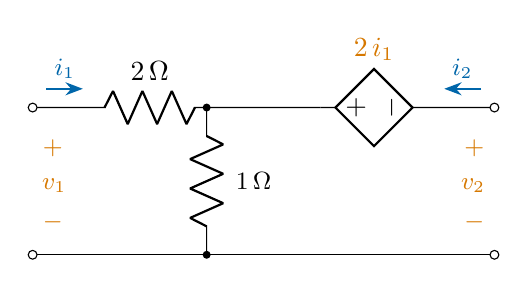
\begin{tikzpicture}[scale=0.85]
  \exTee{0}{$2\ohm$}{$1\ohm$}
\end{tikzpicture}
\end{center}
This is the two-port of Example 14.2. Find $\Hm$.
\end{examplebox}

\solution

\solstep{1}{Port 2 shorted: $\vtwo = 0$}
\begin{minipage}[c]{0.56\linewidth}
\centering
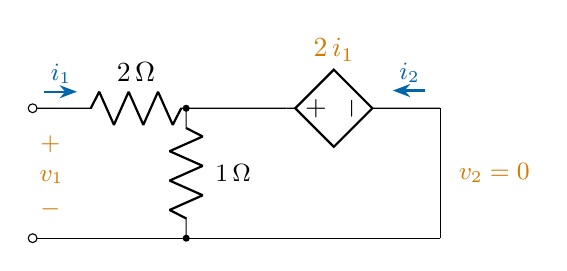
\begin{tikzpicture}[scale=0.75]
  \exTee{3}{$2\ohm$}{$1\ohm$}
\end{tikzpicture}
\end{minipage}\hfill
\begin{minipage}[c]{0.4\linewidth}
Mesh 2 contains the dependent source and $1\ohm$:
\[
  -2\,\ione + (\ione + \itwo) = 0
\]
\[
  \Rightarrow\ \itwo = \ione .
\]
\end{minipage}

\smallskip
Mesh 1 then gives
\[
  \vone = 2\,\ione + (\ione + \itwo) = 4\,\ione .
\]
So $h_{11} = 4\ohm$ and $h_{21} = 1$.

\solstep{2}{Port 1 open: $\ione = 0$}
\begin{minipage}[c]{0.56\linewidth}
\centering
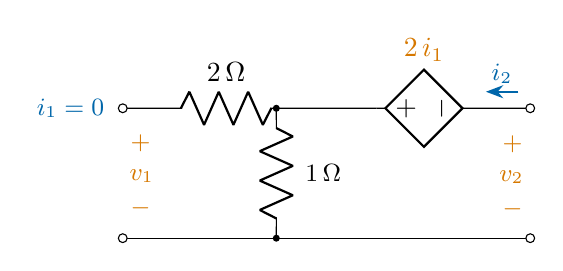
\begin{tikzpicture}[scale=0.75]
  \exTee{2}{$2\ohm$}{$1\ohm$}
\end{tikzpicture}
\end{minipage}\hfill
\begin{minipage}[c]{0.4\linewidth}
The dependent source is $2\,\ione = 0$, a short circuit, and no current flows in $2\ohm$:
\[
  \vtwo = 1 \cdot \itwo \ \Rightarrow\ \itwo = \vtwo .
\]
\end{minipage}

\smallskip
The voltage of port 1 is the voltage of $1\ohm$:
\[
  \vone = \itwo = \vtwo .
\]
So $h_{12} = 1$ and $h_{22} = 1\,\mathrm{S}$.

\solstep{3}{The matrix}
\[
  \Hm = \begin{bmatrix} 4 & 1\\ 1 & 1 \end{bmatrix} .
\]
Check: Example 14.2 gives $\Rm = \left[\begin{smallmatrix} 3 & 1\\ -1 & 1 \end{smallmatrix}\right]$.
Solving its second row for $\itwo$ and substituting into the first row gives the same $\Hm$.
\ \yes

\solstep{4}{The other hybrid matrix}
$\det \Hm = 4 - 1 = 3$, so
\[
  \Hm' = \Hm^{-1} = \frac13 \begin{bmatrix} 1 & -1\\ -1 & 4 \end{bmatrix}
       = \begin{bmatrix} \frac13 & -\frac13\\[2pt] -\frac13 & \frac43 \end{bmatrix} .
\]
Check with the tests of $\Hm'$. Port 2 open: $\vone = 3\,\ione$ and $\vtwo = -\ione$, so
$h'_{11} = \frac13\,\mathrm{S}$ and $h'_{21} = -\frac13$. Port 1 shorted: $3\,\ione + \itwo = 0$
and $\vtwo = -\ione + \itwo = \frac43\,\itwo$, so $h'_{12} = -\frac13$ and
$h'_{22} = \frac43\ohm$. \ \yes

\bigskip
\begin{examplebox}[Example 14.5 --- the hybrid matrix of the ideal transformer]
\begin{minipage}[c]{0.5\linewidth}
\centering
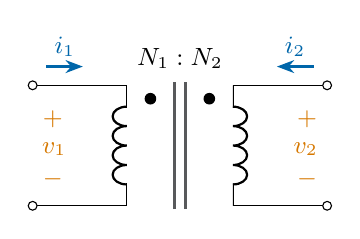
\begin{tikzpicture}[scale=0.85]
  \exXf
\end{tikzpicture}
\end{minipage}\hfill
\begin{minipage}[c]{0.46\linewidth}
The ideal transformer $N_1 : N_2$ (previously) satisfies
\[
  \frac{\vone}{N_1} = \frac{\vtwo}{N_2}, \qquad N_1\,\ione + N_2\,\itwo = 0 .
\]
Find $\Hm$. Does $\Rm$ exist?
\end{minipage}
\end{examplebox}

\solution

\solstep{1}{Solve for $\vone$ and $\itwo$}
With the turns ratio $n = N_1/N_2$:
\[
  \vone = n\,\vtwo, \qquad \itwo = -n\,\ione .
\]

\solstep{2}{The matrix}
\[
  \begin{bmatrix} \vone\\ \itwo \end{bmatrix}
  = \begin{bmatrix} 0 & n\\ -n & 0 \end{bmatrix}
    \begin{bmatrix} \ione\\ \vtwo \end{bmatrix}
  \qquad\Rightarrow\qquad
  \Hm = \begin{bmatrix} 0 & n\\ -n & 0 \end{bmatrix} .
\]
Its inverse is the other hybrid matrix:
\[
  \Hm' = \Hm^{-1} = \begin{bmatrix} 0 & -1/n\\ 1/n & 0 \end{bmatrix} .
\]

\solstep{3}{No resistance matrix}
With both ports open, $\ione = \itwo = 0$, but $\vone = n\,\vtwo$ can take any value. So the
voltages are not determined by the currents: $\Rm$ does not exist. In the same way, shorting
both ports ($\vone = \vtwo = 0$) leaves $\ione = -\itwo/n$ free, so $\Gm$ does not exist either.

%==============================================================
\section{The transmission matrix}

\begin{definitionbox}{Transmission matrix (chain parameters)}
\begin{minipage}[c]{0.46\linewidth}
\[
  \begin{bmatrix} \vone\\ \ione \end{bmatrix}
  = \underbrace{\begin{bmatrix} A & B\\ C & D \end{bmatrix}}_{\Tm}
    \begin{bmatrix} \vtwo\\ -\itwo \end{bmatrix}
\]
\end{minipage}\hfill
\begin{minipage}[c]{0.5\linewidth}
Port 1 in terms of port 2. The minus sign makes $-\itwo$ the current that leaves port 2, for
example towards a load.
\end{minipage}
\end{definitionbox}

\medskip
\begin{examplebox}[Example 14.6 --- the transmission matrix of the ideal transformer]
\begin{minipage}[c]{0.5\linewidth}
\centering
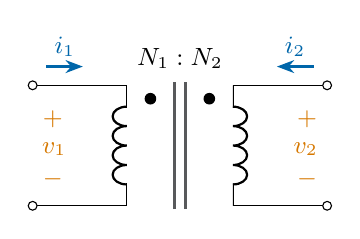
\begin{tikzpicture}[scale=0.85]
  \exXf
\end{tikzpicture}
\end{minipage}\hfill
\begin{minipage}[c]{0.46\linewidth}
Find $\Tm$ for the ideal transformer $N_1 : N_2$.
\end{minipage}
\end{examplebox}

\solution

\solstep{1}{Port 1 in terms of port 2}
From the two transformer equations:
\[
  \vone = \frac{N_1}{N_2}\,\vtwo, \qquad
  \ione = -\frac{N_2}{N_1}\,\itwo = \frac{N_2}{N_1}\,(-\itwo) .
\]

\solstep{2}{The matrix}
\[
  \begin{bmatrix} \vone\\ \ione \end{bmatrix}
  = \begin{bmatrix} N_1/N_2 & 0\\ 0 & N_2/N_1 \end{bmatrix}
    \begin{bmatrix} \vtwo\\ -\itwo \end{bmatrix}
  \qquad\Rightarrow\qquad
  \Tm = \begin{bmatrix} N_1/N_2 & 0\\ 0 & N_2/N_1 \end{bmatrix} .
\]

\subsection*{Which test? Open or short}

Every matrix has two \emph{inputs}: the variables in the vector on the right-hand side. To get
one column, set the other input to zero. A zero current means that port is \textbf{open}; a
zero voltage means that port is \textbf{shorted}. (This is the same as killing a source: a dead
current source is an open, a dead voltage source is a short.)

\begin{center}
\small
\renewcommand{\arraystretch}{1.35}
\begin{tabular}{@{}l c c c@{}}
\toprule
\textbf{Matrix} & \textbf{Inputs} & \textbf{1st column} & \textbf{2nd column}\\
\midrule
$\Rm$: \ $[\,\vone \ \vtwo\,]^T = \Rm\,[\,\ione \ \itwo\,]^T$ & $\ione$, $\itwo$ & $\itwo = 0$: port 2 \textbf{open} & $\ione = 0$: port 1 \textbf{open}\\
$\Gm$: \ $[\,\ione \ \itwo\,]^T = \Gm\,[\,\vone \ \vtwo\,]^T$ & $\vone$, $\vtwo$ & $\vtwo = 0$: port 2 \textbf{shorted} & $\vone = 0$: port 1 \textbf{shorted}\\
$\Hm$: \ $[\,\vone \ \itwo\,]^T = \Hm\,[\,\ione \ \vtwo\,]^T$ & $\ione$, $\vtwo$ & $\vtwo = 0$: port 2 \textbf{shorted} & $\ione = 0$: port 1 \textbf{open}\\
$\Hm'$: \ $[\,\ione \ \vtwo\,]^T = \Hm'\,[\,\vone \ \itwo\,]^T$ & $\vone$, $\itwo$ & $\itwo = 0$: port 2 \textbf{open} & $\vone = 0$: port 1 \textbf{shorted}\\
$\Tm$: \ $[\,\vone \ \ione\,]^T = \Tm\,[\,\vtwo \ {-\itwo}\,]^T$ & $\vtwo$, $-\itwo$ & $\itwo = 0$: port 2 \textbf{open} & $\vtwo = 0$: port 2 \textbf{shorted}\\
\bottomrule
\end{tabular}
\end{center}

The names already say it: $\Rm$ is the open-circuit matrix and $\Gm$ the short-circuit matrix.
$\Hm$ mixes a current and a voltage as inputs, so its tests are mixed too, and its entries have
mixed units. $\Tm$ is the odd one: both tests are done at port 2, and port 1 is only measured.
The port that is not zeroed is driven by a source of its own input type: a current source if
its input is a current, a voltage source if it is a voltage.

%==============================================================
\section{When does a matrix exist?}\label{sec:exist}

Each matrix makes a promise: \emph{choose its two inputs freely, and the two outputs are then
fixed}. Some two-ports break this promise for some matrices. Then that matrix does not exist.

\subsection{The test: both inputs zero}

Set both inputs to zero at the same time.
\begin{itemize}[itemsep=3pt]
  \item If the circuit then forces all four port variables to zero, the matrix \textbf{exists}.
  \item If some port variable can still be nonzero, the matrix \textbf{does not exist}.
\end{itemize}
Why: a nonzero solution with zero inputs can be added to any other solution. The inputs stay
the same, but the outputs change. So the inputs do not fix the outputs.

\begin{center}
\small
\renewcommand{\arraystretch}{1.35}
\begin{tabular}{@{}l l l@{}}
\toprule
\textbf{Matrix} & \textbf{Inputs set to zero} & \textbf{In the circuit}\\
\midrule
$\Rm$ & $\ione = \itwo = 0$ & both ports \textbf{open}\\
$\Gm$ & $\vone = \vtwo = 0$ & both ports \textbf{shorted}\\
$\Hm$ & $\ione = 0$, $\vtwo = 0$ & port 1 open, port 2 shorted\\
$\Hm'$ & $\vone = 0$, $\itwo = 0$ & port 1 shorted, port 2 open\\
$\Tm$ & $\vtwo = 0$, $\itwo = 0$ & port 2 \textbf{open and shorted}: no voltage, no current\\
\bottomrule
\end{tabular}
\end{center}
For $\Tm$ both conditions are at port 2. Port 1 is left alone. If port 1 can still carry a
current or a voltage, port 2 cannot tell what happens at port 1, and $\Tm$ does not exist.

\subsection{Three simple cases}

\begin{minipage}[t]{0.47\linewidth}
\centering
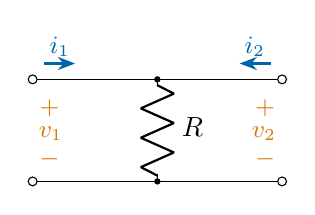
\begin{tikzpicture}[scale=0.72]
  \draw (0,1.8) -- (4.4,1.8); \draw (0,0) -- (4.4,0);
  \draw (2.2,1.8) to[R, l=$R$] (2.2,0);
  \fill (2.2,1.8) circle (1.6pt); \fill (2.2,0) circle (1.6pt);
  \pone{0}{1.8} \ptwo{4.4}{1.8}
\end{tikzpicture}\\[2pt]
{\small (a) one resistor across both ports}
\end{minipage}\hfill
\begin{minipage}[t]{0.47\linewidth}
\centering
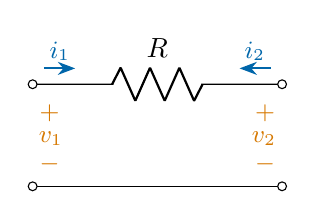
\begin{tikzpicture}[scale=0.72]
  \draw (0,1.8) to[R, l=$R$] (4.4,1.8); \draw (0,0) -- (4.4,0);
  \pone{0}{1.8} \ptwo{4.4}{1.8}
\end{tikzpicture}\\[2pt]
{\small (b) one resistor between the ports}
\end{minipage}

\medskip
\textbf{(a) No $\Gm$.} Short both ports. The two shorts and the wires form a loop around the
resistor. A current can enter port 1 and leave port 2 through the wires: $\ione = -\itwo$ can be
anything. So $\Gm$ does not exist. $\Rm$ does exist:
\[
  \vone = \vtwo = R\,(\ione + \itwo)
  \qquad\Rightarrow\qquad
  \Rm = \begin{bmatrix} R & R\\ R & R \end{bmatrix}, \qquad \det \Rm = 0 .
\]
$\Rm$ is not invertible, as it must be: if $\Gm$ existed, it would be $\Rm^{-1}$.

\textbf{(b) No $\Rm$.} Open both ports. Nothing connects the top terminals to the bottom
ones, so $\vone = \vtwo$ can be any value. So $\Rm$ does not exist. $\Gm$ does exist:
\[
  \ione = -\itwo = \frac{\vone - \vtwo}{R}
  \qquad\Rightarrow\qquad
  \Gm = \frac1R\begin{bmatrix} 1 & -1\\ -1 & 1 \end{bmatrix}, \qquad \det \Gm = 0 .
\]

\textbf{(c) No $\Tm$: two separate resistors (Example 14.1).} Make port 2 dead: $\vtwo = 0$ and
$\itwo = 0$. The $2\ohm$ resistor at port 1 does not notice: any $\ione$ with $\vone = 2\,\ione$ is
still possible. So $\Tm$ does not exist. In words: port 2 knows nothing about port 1, so port 1
cannot be written in terms of port 2.

The ideal transformer (Example 14.5) has neither $\Rm$ nor $\Gm$, but $\Hm$, $\Hm'$ and $\Tm$
exist. Cases (a) and (b) both have $\Tm$: $\left[\begin{smallmatrix} 1 & 0\\ 1/R & 1 \end{smallmatrix}\right]$
and $\left[\begin{smallmatrix} 1 & R\\ 0 & 1 \end{smallmatrix}\right]$.

\subsection{From one matrix to another}

When one matrix is known, the others follow by solving its two equations for the other
variables. Each step divides by one number, and that number must not be zero. For example,
$\Tm$ from $\Rm$: the second row $\vtwo = r_{21}\,\ione + r_{22}\,\itwo$ gives
\[
  \ione = \frac{1}{r_{21}}\,\vtwo + \frac{r_{22}}{r_{21}}\,(-\itwo)
  \qquad\text{(needs } r_{21} \neq 0\text{)},
\]
and the first row then gives $\vone$. The result is
\[
  \Tm = \frac{1}{r_{21}} \begin{bmatrix} r_{11} & \det \Rm\\ 1 & r_{22} \end{bmatrix} .
\]
The other cases work the same way:
\begin{center}
\small
\renewcommand{\arraystretch}{1.4}
\begin{tabular}{@{}>{\raggedright}p{2.9cm} >{\raggedright}p{2.2cm} >{\raggedright\arraybackslash}p{7.2cm}@{}}
\toprule
\textbf{Wanted} & \textbf{Needs} & \textbf{If it fails}\\
\midrule
$\Gm = \Rm^{-1}$ & $\det \Rm \neq 0$ & with both ports shorted a current can still flow (case a)\\
$\Hm$ from $\Rm$ & $r_{22} \neq 0$ & with port 1 open, port 2 is a short: $\vtwo$ cannot be chosen\\
$\Hm'$ from $\Rm$ & $r_{11} \neq 0$ & with port 2 open, port 1 is a short: $\vone$ cannot be chosen\\
$\Hm' = \Hm^{-1}$ & $\det \Hm \neq 0$ & $\vone$ and $\itwo$ cannot both be chosen freely\\
$\Tm$ from $\Rm$ & $r_{21} \neq 0$ & port 1 has no effect on port 2 (case c)\\
$\Tm$ from $\Gm$ & $g_{21} \neq 0$ & port 1 has no effect on port 2\\
\bottomrule
\end{tabular}
\end{center}
The formulas:
\[
  \Hm = \frac{1}{r_{22}} \begin{bmatrix} \det \Rm & r_{12}\\ -r_{21} & 1 \end{bmatrix}, \qquad
  \Hm' = \frac{1}{r_{11}} \begin{bmatrix} 1 & -r_{12}\\ r_{21} & \det \Rm \end{bmatrix}, \qquad
  \Tm = -\frac{1}{g_{21}} \begin{bmatrix} g_{22} & 1\\ \det \Gm & g_{11} \end{bmatrix} .
\]
Check with Example 14.2: $\Rm = \left[\begin{smallmatrix} 3 & 1\\ -1 & 1 \end{smallmatrix}\right]$,
$\det \Rm = 4$, $r_{22} = 1$, so $\Hm = \left[\begin{smallmatrix} 4 & 1\\ 1 & 1 \end{smallmatrix}\right]$,
as found before. And $r_{21} = -1 \neq 0$, so $\Tm$ exists:
$\Tm = -\left[\begin{smallmatrix} 3 & 4\\ 1 & 1 \end{smallmatrix}\right]$.

%==============================================================
\section{Measuring a two-port}

In a laboratory the two-port is a closed box with four terminals. Nothing inside is known, but
if it is linear, $\Rm$ (or $\Gm$, $\Hm$, $\Tm$) has only four numbers. Each experiment gives two
equations, so \textbf{two experiments} are enough. The open- and short-circuit tests are the
two experiments that give the entries most directly.

\subsection{Ideal meters are opens and shorts}

An ideal \textbf{voltmeter} draws no current: it is an \emph{open} circuit. An ideal
\textbf{ammeter} has no voltage across it: it is a \emph{short} circuit. So
\begin{itemize}
  \item a port with only a voltmeter across it is an \textbf{open} port, and the meter reads
        its voltage;
  \item a port closed by only an ammeter is a \textbf{shorted} port, and the meter reads its
        current.
\end{itemize}
The tests of this lecture are therefore real experiments: a source at one port, and meters at
both ports.

\medskip
\noindent
\begin{minipage}[t]{0.49\linewidth}
\centering
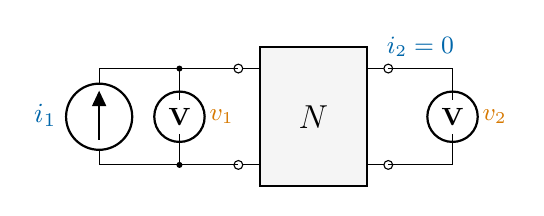
\begin{tikzpicture}[scale=0.68]
  \bench{0}
\end{tikzpicture}\\[2pt]
{\small\raggedright \textbf{Open-circuit test.} A current source drives port 1; voltmeters read
$\vone$ and $\vtwo$. Then $r_{11} = \vone/\ione$ and $r_{21} = \vtwo/\ione$.}
\end{minipage}\hfill
\begin{minipage}[t]{0.49\linewidth}
\centering
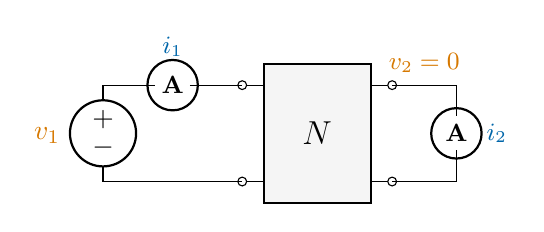
\begin{tikzpicture}[scale=0.68]
  \bench{1}
\end{tikzpicture}\\[2pt]
{\small\raggedright \textbf{Short-circuit test.} A voltage source drives port 1; ammeters read
$\ione$ and $\itwo$. Then $g_{11} = \ione/\vone$ and $g_{21} = \itwo/\vone$.}
\end{minipage}

\medskip
Each entry is one meter reading divided by the source value; no circuit analysis is needed.
Moving the source to port 2 gives the second column. For $\Hm$, port 2 gets an ammeter and port
1 a voltmeter, and so on, following the table above.

\subsection{When a port cannot be opened or shorted}

Opening or shorting a port is not always possible. A short at the output of an amplifier may
damage it. An open-circuit test may be impossible: with port 2 of an ideal transformer open,
no current can enter port 1, so its $\Rm$ does not exist. Then any \textbf{two independent experiments} still work. Put the two
measured current vectors side by side, and the two voltage vectors side by side:
\[
  \underbrace{\begin{bmatrix} \vone^{(1)} & \vone^{(2)}\\ \vtwo^{(1)} & \vtwo^{(2)} \end{bmatrix}}_{\mathbf{V}}
  = \Rm\,
  \underbrace{\begin{bmatrix} \ione^{(1)} & \ione^{(2)}\\ \itwo^{(1)} & \itwo^{(2)} \end{bmatrix}}_{\mathbf{I}}
  \qquad\Rightarrow\qquad
  \Rm = \mathbf{V}\,\mathbf{I}^{-1} .
\]
The superscript is the experiment number. The experiments are independent when $\mathbf{I}$ is
invertible. The open-circuit tests are the special case $\mathbf{I}$ diagonal, where no inverse
has to be computed.

\bigskip
\begin{examplebox}[Example 14.7 --- $\Rm$ from two measurements]
Two experiments on a linear two-port give
\begin{center}
\renewcommand{\arraystretch}{1.2}
\begin{tabular}{@{}lcccc@{}}
\toprule
 & $\ione$ (A) & $\itwo$ (A) & $\vone$ (V) & $\vtwo$ (V)\\
\midrule
Experiment 1 & $1$ & $1$ & $5$ & $5$\\
Experiment 2 & $1$ & $-1$ & $3$ & $-1$\\
\bottomrule
\end{tabular}
\end{center}
Neither experiment has an open port. Find $\Rm$.
\end{examplebox}

\solution

\solstep{1}{Stack the experiments}
\[
  \begin{bmatrix} 5 & 3\\ 5 & -1 \end{bmatrix}
  = \Rm \begin{bmatrix} 1 & 1\\ 1 & -1 \end{bmatrix} .
\]

\solstep{2}{Solve}
$\det \mathbf{I} = -2 \neq 0$, so the experiments are independent, and
\[
  \mathbf{I}^{-1} = \frac12 \begin{bmatrix} 1 & 1\\ 1 & -1 \end{bmatrix},
  \qquad
  \Rm = \begin{bmatrix} 5 & 3\\ 5 & -1 \end{bmatrix} \cdot \frac12
        \begin{bmatrix} 1 & 1\\ 1 & -1 \end{bmatrix}
      = \begin{bmatrix} 4 & 1\\ 2 & 3 \end{bmatrix} .
\]

\solstep{3}{Check}
Experiment 1: $\Rm\,[\,1 \ 1\,]^T = [\,5 \ 5\,]^T$. Experiment 2:
$\Rm\,[\,1 \ {-1}\,]^T = [\,3 \ {-1}\,]^T$. \ \yes

%==============================================================
\section{The power of a two-port}

Let $P_N$ be the sum of the powers absorbed by all elements inside the two-port $N$.

\begin{ideabox}[Theorem]
\[
  P_N = \vone\,\ione + \vtwo\,\itwo .
\]
\end{ideabox}

\textbf{Why.} Connect sources to the two ports. By Tellegen's theorem (previously), the sum of
the absorbed powers of all branches is zero. The port sources absorb $-\vone\,\ione$ and
$-\vtwo\,\itwo$, so the elements inside $N$ absorb $\vone\,\ione + \vtwo\,\itwo$.

\begin{definitionbox}{Passive and active two-ports}
A two-port is \textbf{passive} if $P_N \geq 0$ for all possible port variables
$(\vone, \ione, \vtwo, \itwo)$. It is \textbf{active} if it is not passive.
\end{definitionbox}

\medskip
\begin{examplebox}[Example 14.8 --- is the ideal transformer passive?]
\begin{minipage}[c]{0.5\linewidth}
\centering
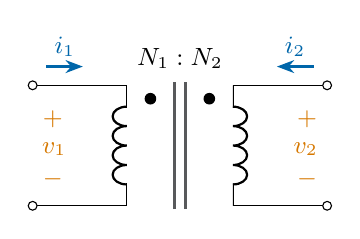
\begin{tikzpicture}[scale=0.85]
  \exXf
\end{tikzpicture}
\end{minipage}\hfill
\begin{minipage}[c]{0.46\linewidth}
Find the power $P_N$ of the ideal transformer. Is it passive or active?
\end{minipage}
\end{examplebox}

\solution

\solstep{1}{The power}
Plug $\vone = n\,\vtwo$ and $\itwo = -n\,\ione$ into the theorem:
\[
  P_N = \vone\,\ione + \vtwo\,\itwo = n\,\vtwo\,\ione - n\,\vtwo\,\ione = 0 .
\]

\solstep{2}{Passive or active}
$P_N = 0 \geq 0$ for all port variables, so the ideal transformer is passive. It neither
absorbs nor delivers power: what enters one port leaves the other.

%==============================================================
\section*{Summary}

\begin{center}
\small
\renewcommand{\arraystretch}{1.3}
\begin{tabular}{@{}>{\raggedright}p{2.6cm} >{\raggedright}p{4.5cm} >{\raggedright\arraybackslash}p{6.4cm}@{}}
\toprule
\textbf{Matrix} & \textbf{Equation} & \textbf{How to find it}\\
\midrule
resistance $\Rm$ & $[\,\vone \ \vtwo\,]^T = \Rm\,[\,\ione \ \itwo\,]^T$ & KVL, or open-circuit tests ($\itwo = 0$, then $\ione = 0$)\\
conductance $\Gm$ & $[\,\ione \ \itwo\,]^T = \Gm\,[\,\vone \ \vtwo\,]^T$ & short-circuit tests; $\Gm = \Rm^{-1}$ when both exist\\
hybrid $\Hm$, $\Hm'$ & $[\,\vone \ \itwo\,]^T = \Hm\,[\,\ione \ \vtwo\,]^T$ & port 2 shorted, then port 1 open; $\Hm' = \Hm^{-1}$\\
transmission $\Tm$ & $[\,\vone \ \ione\,]^T = \Tm\,[\,\vtwo \ {-\itwo}\,]^T$ & port 1 in terms of port 2\\
existence & set both inputs to zero & exists if all port variables are then forced to zero\\
power & $P_N = \vone\,\ione + \vtwo\,\itwo$ & passive if $P_N \geq 0$ for all port variables\\
\bottomrule
\end{tabular}
\end{center}

\clearpage
\appendix
\section{Passivity from the matrix}

A two-port is passive if $P_N \geq 0$ for all port variables. When $\Rm$, $\Gm$ or $\Hm$ exists,
this can be decided from the matrix alone.

\subsection{Power as a quadratic form}

Write $\mathbf{i} = [\,\ione \ \itwo\,]^T$ and $\mathbf{v} = [\,\vone \ \vtwo\,]^T$. With
$\mathbf{v} = \Rm\,\mathbf{i}$,
\[
  P_N = \vone\,\ione + \vtwo\,\itwo = \mathbf{i}^T\mathbf{v} = \mathbf{i}^T \Rm\,\mathbf{i}
      = r_{11}\,\ione^2 + (r_{12} + r_{21})\,\ione\,\itwo + r_{22}\,\itwo^2 .
\]
Only the sum $r_{12} + r_{21}$ appears. So only the \textbf{symmetric part} of $\Rm$ matters:
\[
  \Rm_s = \tfrac12\,(\Rm + \Rm^T)
        = \begin{bmatrix} r_{11} & \tfrac12(r_{12} + r_{21})\\[2pt]
                          \tfrac12(r_{12} + r_{21}) & r_{22} \end{bmatrix},
  \qquad P_N = \mathbf{i}^T \Rm_s\,\mathbf{i} .
\]

\subsection{The test}

\begin{ideabox}[Passivity test]
The two-port is passive if and only if $\Rm_s$ is positive semidefinite. For a $2 \times 2$
matrix this means
\[
  r_{11} \geq 0, \qquad r_{22} \geq 0, \qquad
  r_{11}\,r_{22} - \tfrac14\,(r_{12} + r_{21})^2 \geq 0 .
\]
If one condition fails, some port currents give $P_N < 0$: the two-port is active.
\end{ideabox}

The same works with the other matrices. With $\Gm$, $P_N = \mathbf{v}^T \Gm\,\mathbf{v}$: test
$\frac12(\Gm + \Gm^T)$. With $\Hm$, take $\mathbf{x} = [\,\ione \ \vtwo\,]^T$; then
$[\,\vone \ \itwo\,]^T = \Hm\,\mathbf{x}$ and $P_N = \mathbf{x}^T \Hm\,\mathbf{x}$: test
$\frac12(\Hm + \Hm^T)$. The transmission matrix $\Tm$ does not give such a form, because it
relates port 1 to port 2 instead of the voltages to the currents.

\bigskip
\begin{examplebox}[Example A.1 --- the two-port of Example 14.4]
$\Rm = \begin{bmatrix} 3 & 1\\ -1 & 1 \end{bmatrix}$. It contains a dependent source. Is it
passive?
\end{examplebox}

\solution

\solstep{1}{The symmetric part}
\[
  \Rm_s = \begin{bmatrix} 3 & 0\\ 0 & 1 \end{bmatrix} .
\]

\solstep{2}{The test}
$3 \geq 0$, $1 \geq 0$ and $3 \cdot 1 - 0^2 = 3 \geq 0$. The two-port is \textbf{passive}: a
dependent source inside does not make a two-port active by itself.

\bigskip
\begin{examplebox}[Example A.2 --- the ideal transformer]
$\Hm = \begin{bmatrix} 0 & n\\ -n & 0 \end{bmatrix}$ (Example 14.5). Is it passive?
\end{examplebox}

\solution

\solstep{1}{The symmetric part}
$\Hm$ is antisymmetric, $\Hm^T = -\Hm$, so $\frac12(\Hm + \Hm^T) = \mathbf{0}$.

\solstep{2}{The test}
$P_N = 0$ for all port variables: the transformer is \textbf{passive} and absorbs no power, as
in Example 14.8.

\bigskip
\begin{examplebox}[Example A.3 --- a larger gain]
\begin{minipage}[c]{0.56\linewidth}
\centering
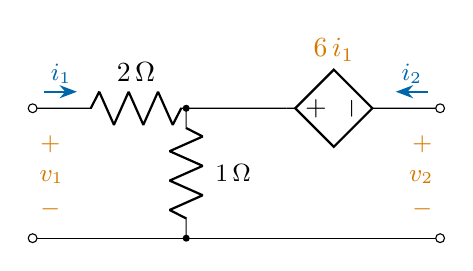
\begin{tikzpicture}[scale=0.75]
  \exTee[6]{0}{$2\ohm$}{$1\ohm$}
\end{tikzpicture}
\end{minipage}\hfill
\begin{minipage}[c]{0.4\linewidth}
The circuit of Example 14.2 with the dependent source $6\,\ione$ instead of $2\,\ione$. Is it
passive?
\end{minipage}
\end{examplebox}

\solution

\solstep{1}{The matrix}
As in Example 14.2, with $2$ replaced by $6$:
\[
  \Rm = \begin{bmatrix} 3 & 1\\ 1 - 6 & 1 \end{bmatrix}
      = \begin{bmatrix} 3 & 1\\ -5 & 1 \end{bmatrix},
  \qquad
  \Rm_s = \begin{bmatrix} 3 & -2\\ -2 & 1 \end{bmatrix} .
\]

\solstep{2}{The test}
$3 \cdot 1 - (-2)^2 = -1 < 0$: the two-port is \textbf{active}.

\solstep{3}{A check}
Take $\ione = 1\A$ and $\itwo = 2\A$:
\[
  P_N = 3 \cdot 1^2 + (1 - 5) \cdot 1 \cdot 2 + 1 \cdot 2^2 = -1\,\mathrm{W} .
\]
The two-port delivers $1\,\mathrm{W}$ to the outside. \ \yes

\end{document}
